\documentclass[a4paper]{jpconf}
\usepackage{graphicx}

\usepackage{amsmath}
\usepackage{bm}


\begin{document}
\title{Numerical calculation of spectral problems in SP$_3$ approximation by FEM}

\author{Alexander O. Vasilev}

\address{North-Eastern Federal University, 58, Belinskogo, Yakutsk, Russia}

\ead{haska87@gmail.com}

\begin{abstract}
The SP$_3$ approximation of the neutron transport equation allows improving the accuracy for both static and transient simulations for reactor core analysis compared with the neutron diffusion theory. 
Besides, the SP$_3$ calculation costs are much less than higher order transport methods ($\mathrm{S_N}$ or $\mathrm{P_N}$). 
Another advantage of the SP$_3$ approximation is a similar structure of equations that is used in the diffusion method. 
Therefore, there is no difficulty to implement the SP$_3$ solution option to the multi-group neutron diffusion codes. 
In this work, the application of the SP$_3$ methodology based on solution of the $\lambda$- and $\alpha$-spectral problems has been tested for reactor benchmarks. 
The FEM is chosen to achieve the geometrical generality. 
The results calculated with the diffusion and SP$_3$ methods are compared with the reference calculation results.
\end{abstract}

\section{Introduction}
The diffusion approximation of the neutron transport equation is widely used in nuclear reactor analysis allowing whole-core calculations with reasonable accuracy. 
The $\mathrm{SP_3}$ \cite{brantley2000simplified} method can be considered as an improved approximation of the neutron transport equation compared with the diffusion method. 
In this regard, it will be very useful to compare the spectral parameters, calculated by both the diffusion and $\mathrm{SP_3}$ methods. 

To characterize the reactor steady-state conditions or dynamic behavior, some spectral problems are considered \cite{bell1970, stacey2007}. 
The steady-state condition is usually described by solution of a spectral problem ($\lambda$-eigenvalue problem); the fundamental eigenvalue (the largest eigenvalue) is called k-effective of the reactor core. 
The reactor dynamic behavior can naturally be described on the basis of the approximate solution expansion in time-eigenvalue of $\alpha$-eigenvalue problem \cite{bell1970}. 
At large times, one can talk about the asymptotic behavior of a neutron flux, whose amplitude is exp($\alpha$t). 
Previously the complex eigenvalues and eigenfunctions were found in the spectral problems for some numerical tests \cite{avvakumov2017spectral}.

\section{Problem statement}
Let’s consider the symmetric form of the $\mathrm{SP_3}$ equation for the neutron flux \cite{ryu2013fem}.
The neutron dynamics is considered in the limited convex two-dimensional or three-dimensional area  $\Omega$ ($\bm x = \{x_1, ..., x_d\} \in \Omega, \ d = 2,3$) with boundary $\partial \Omega$. 
The neutron transport is described by the system of equations
\begin{equation}\label{1.1}
\begin{split}
 \frac{1}{v_g} \frac{\partial \phi_{0,g}}{\partial t} - \frac{2}{v_g} \frac{\partial \phi_{2,g}}{\partial t} - & \nabla \cdot D_{0,g} \nabla \phi_{0,g} + \Sigma_{r,g} \phi_{0,g} -  2\Sigma_{r,g} \phi_{2,g} = \\ 
 =  & (1-\beta)\chi_{n,g} S_{n} + S_{s,g} + \chi_{d,g} S_d, \\
 -\frac{2}{v_g} \frac{\partial \phi_{0,g}}{\partial t} + \frac{9}{v_g} \frac{\partial \phi_{2,g}}{\partial t} - & \nabla \cdot D_{2,g} \nabla \phi_{2,g} + (5\Sigma_{t,g} + 4\Sigma_{r,g}) \phi_{2,g} - 2\Sigma_{r,g} \phi_{0,g} = \\ 
 =  & -2(1-\beta)\chi_{n,g} S_{n} - 2S_{s,g} - 2\chi_{d,g} S_d,
\end{split}
\end{equation}
where
\[
S_{n} =  \sum_{g'=1}^{G} \nu \Sigma_{f,g'} \phi_{g'}, 
\quad
S_{s,g} = \sum_{g\neq g'=1}^{G} \Sigma_{s,g'\rightarrow g} \phi_{g'},
\quad
S_{d} = \sum_{m=1}^{M} \lambda_m c_m,
\]
\[
\phi_{0,g}=\phi_g + 2\phi_{2,g}, 
\quad
D_{0,g} = \cfrac{1}{3\Sigma_{tr,g}}, 
\quad
D_{2,g} = \cfrac{9}{7\Sigma_{t,g}}, 
\quad g=1,2,...,G.
\]
Here $G$ --- number of energy groups,
$\phi_g(\bm x, t)$ --- scalar flux,
$\phi_{0,g}(\bm x, t)$ --- 0th moment of angular flux,
$\phi_{2,g}(\bm x, t)$ --- 2th moment of angular flux,
$\Sigma_{t,g}(\bm x, t)$ --- total cross-section, 
$\Sigma_{tr,g}(\bm x, t)$ --- transport cross-section, 
$\Sigma_{r,g}(\bm x, t)$ --- removal cross-section,
$\Sigma_{s,g'\rightarrow g}(\bm x, t)$ --- scattering cross-section,
$\chi_g$  --- spectra of neutrons, 
$\nu\Sigma_{f,g}(\bm x, t)$ --- generation cross-section,
$c_m(\bm x, t)$ --- density of sources of delayed neutrons,
$\lambda_m$ --- decay constant of sources of delayed neutrons,
$M$ --- number of types of delayed neutrons.

The density of sources of delayed neutrons is described by the equations
\begin{equation}\label{1.2}
 \frac{\partial c_m}{\partial t} + \lambda_m c_m = \beta_m S_{n},
 \quad m = 1,2, ..., M, 
\end{equation}
where $\beta_m$ is the fraction of delayed neutrons of m-type, and
$
 \beta = \sum_{m=1}^{M} \beta_m.
$
The Marshak-type conditions are set at the boundary of the area $\partial \Omega$
\begin{equation}\label{1.3}
\begin{split}
\begin{bmatrix}
J_{0,g}(\bm x)\\
J_{2,g}(\bm x)\\
\end{bmatrix}
=
\begin{bmatrix}
\phantom{-}\cfrac{1}{2} & -\cfrac{3}{8} \\
 -\cfrac{3}{8} & \phantom{-}\cfrac{21}{8} \\
\end{bmatrix}
\begin{bmatrix}
\phi_{0,g}(\bm x) \\
\phi_{2,g}(\bm x) \\
\end{bmatrix},
\quad
J_{i,g}(\bm x) = -D_{i,g}\nabla\phi_{i,g}(\bm x), 
\quad
i = 0, 2.
\end{split}
\end{equation}

System of equations (\ref{1.1}) and (\ref{1.2}) is supplemented with boundary conditions (\ref{1.3}) and corresponding initial conditions
\begin{equation}\label{1.4}
 \phi_g(\bm x,0) = \phi_g^0(\bm x), 
 \quad g = 1,2, ..., G,
 \quad c_m(\bm x,0) = c_m^0(\bm x), 
 \quad m = 1,2, ..., M.
\end{equation}

Let's write the boundary problem (\ref{1.1})--(\ref{1.4}) in operator form. 
The vectors $\bm u_1 = \{\phi_{0,1}, \phi_{0,2}, \cdots, \phi_{0,G}\}$, $\bm u_2 = \{\phi_{2,1}, \phi_{2,2}, \cdots, \phi_{2,G}\}$, $\bm c = \{c_1, c_2, ..., c_M\}$ and matrices are defined as follows
\[
V = (\mathrm{v}_{gg'}),
\enskip
\mathrm{v}_{gg'} = \frac{1}{v_g} \delta_{gg'},
\quad
B = (b_{gg'}),
\enskip
b_{gg} = -2\Sigma_{r,g},
\enskip
b_{gg'} = 2\Sigma_{s, g' \rightarrow g},
\]
\[
A_1 = (a_{gg'}),
\enskip
a_{gg} = -\nabla \cdot D_{0,g} \nabla + \Sigma_{r,g},
\enskip
a_{gg'} = -\Sigma_{s, g' \rightarrow g},
\]
\[
A_2 = (a_{gg'}),
\enskip
a_{gg} = -\nabla \cdot D_{2,g} \nabla + 5\Sigma_{tr,g} + 4\Sigma_{r,g},
\enskip
a_{gg'} = -4\Sigma_{s, g' \rightarrow g},
\]
\[
F = (f_{gg'}),
\enskip
f_{gg'} = \chi_{n,g}\nu\Sigma_{f,g'},
\quad
E =(e_{gm}),
\enskip
e_{gm} = \chi_{d,g}\lambda_m,
\]
\[
\Lambda = (\lambda_{mm'}), 
\enskip
\lambda_{mm'} = \delta_{mm'}\lambda_m,
\quad
Q = (q_{mg}),
\enskip
q_{mg} =\beta_m \nu\Sigma_{f,g},
\]
where
$\delta_{g g'}$ is the Kronecker symbol.
We shall use the set of vectors $\bm {u_1, u_2}$, whose components satisfy the boundary conditions (\ref{1.3}). 
Using the set definitions, the system of equations (\ref{1.1}) and (\ref{1.2}) can be written as following
\begin{equation}\label{1.5}
\begin{split}
V (\frac{\partial \bm u_1}{\partial t} - 2 \frac{\partial \bm u_2}{\partial t}) + A_1 \bm u_1 + B \bm u_2 &=(1-\beta) F (\bm u_1 - 2\bm u_2) + E\bm c,
\\
V(- 2 \frac{\partial \bm u_1}{\partial t} + 9 \frac{\partial \bm u_2}{\partial t} ) + A_2 \bm u_2 + B \bm u_1 &=-2(1-\beta) F (\bm u_1 - 2\bm u_2) - 2E\bm c,
\\
\frac{\partial \bm c}{d t} + \Lambda \bm c &= Q (\bm u_1 - 2\bm u_2). 
\end{split}
\end{equation}
The Cauchy problem is formulated for equations (\ref{1.5}) when
\begin{equation}\label{1.7}
 \bm u_1(0) = \bm u_1^0, \quad  \bm u_2(0) = \bm u_2^0, \quad \bm c(0) = \bm c^0,
\end{equation} 
where $\bm u_1^0 = \{\phi_{0,1}^0,  \phi_{0,2}^0, ...,  \phi_{0,G}^0 \}$, 
$\bm u_2^0 = \{\phi_{2,1}^0,  \phi_{2,2}^0, ...,  \phi_{2,G}^0 \}$ and 
$\bm c^0 = \{ c_1^0,  c_2^0, ...,  c_M^0 \}$.

\section{Spectral problems}
The spectral problem, which is known as the $\lambda$-spectral problem, is usually considered.
For the system of equations (\ref{1.5}), we have
\begin{equation}\label{1.8}
L \bm \varphi = \lambda^{(k)} M \bm \varphi,
\end{equation}
where
\[
\bm \varphi = \{\bm \varphi_1, \bm \varphi_2\},
\quad
L = \begin{pmatrix}
A_1 & B \\
B & A_2 \\
\end{pmatrix},
\quad
M = \begin{pmatrix}
F & -2F \\
-2F & 4F \\
\end{pmatrix}.
\]
The minimal eigenvalue is used for characterisation of neutron field, thus $k = 1 /\lambda^{(k)}_1$ is the effective multiplication factor (k-effective).
The value $k = 1$ is related to the critical state of the reactor, and the corresponding eigenfunction $\bm{\varphi}^{(1)}(\bm x)$ is the stationary solution of the Eq (\ref{1.5}).
At $k > 1$, one can speak about supercriticality, at $k < 1$ --- about subcriticality.

The spectral problem (\ref{1.8}) cannot directly be connected with the
dynamic processes in a nuclear reactor. The eigenvalues of the multiplication factor of the reactor and the corresponding eigenfunctions do not depend on the time delay for the emission of delayed neutrons. 
At the best, we can get only the limiting case --- the stationary critical state.
The more acceptable spectral characteristics for the non-stationary equation (\ref{1.5}) are related the spectral problem
\begin{equation}\label{1.9}
\begin{split}
L \bm \varphi - (1 - \beta) M \bm \varphi - I \bm s &= \lambda^{(\alpha)} W \bm \varphi, \\
\Lambda \bm s - R \bm \varphi  &= \lambda^{(\alpha)} \bm s.
\end{split}
\end{equation}
where
\[
I = \begin{pmatrix}
E \\
-2E \\
\end{pmatrix},
\quad
R = \begin{pmatrix}
Q & -2Q \\
\end{pmatrix},
\quad
W = \begin{pmatrix}
V & -2V \\
-2V & 9V \\
\end{pmatrix}
\]
The fundamental eigenvalue $\alpha = \lambda^{(\alpha)}_1$ is called the $\alpha$-eigenvalue or the period eigenvalue, because it is inversely related to the reactor period. If $\alpha = 0$, then the reactor is critical; if $\alpha < 0$ --- supercritical state; if $\alpha > 0$ --- subcritical state.

The problem of the period eigenvalues essentially takes into account the contribution of delayed neutrons.
In particular, the long lifetime of the predecessors of delayed neutrons makes a large contribution to the slowly decreasing eigenfunctions of the reactor period, and this does not occur when only prompt neutrons are taken into account.

The asymptotic behaviour of Cauchy problem solution (\ref{1.5})-(\ref{1.7}) at large times can be connected with the eigenvalue $\alpha$.
In this regular mode, the reactor behaviour is described by the function $\exp(-\alpha t) \bm \varphi^{(1)}(\bm x)$.

\section{IAEA-2D with reflector}
We consider the test IAEA-2D with reflector.
The two-group model ($G = 2$) and one group of delayed neutrons ($M = 1$) are used. 
Description and coefficients are here \cite{chao1995}.

The method of finite elements \cite{brenner2008} on triangular calculation grids is used for the approximate solution of the spectral problems. 
The standard Lagrangian finite elements are used.
The software has been developed using the library FEniCS \cite{logg2012}.
SLEPc has been used for numerical solution of the spectral problems.
We used a Krylov-Schur algorithm with an accuracy of $10^{-15}$.
The following parameters were varied in the calculations:
$n$ --- the number of triangles per one assembly; 
$p$ --- the order of finite element.

In this work we compare the $\mathrm{SP_3}$ calculations with the previous diffusion model calculations \cite{avvakumov2014, avvakumov2015}.

\subsection{Solution of Lambda Modes spectral problem}
As a reference solution we take the solution obtained using the MCNP4C code \cite{bahabadi2016}. 
The maximum difference in assembly power between two models is about 2 percent for the rodded assemblies (material 3).
\begin{table}[htp]
\caption{The effective multiplication factor.}
\label{tab:iaea_with_lambda}
\begin{center}
\begin{tabular}{c c r r r r r r r r}
\hline
$n$ & $p$ & $k_{dif}$ & $\Delta_{dif}$ & $\delta_{dif}$ &$t$ &$k_{sp_3}$& $\Delta_{sp_3}$ & $\delta_{sp_3}$ &$t$ \\
\hline
	& 1	& 1.01041& 418&14.34& 0.01& 1.01159& 536& 14.14 &0.02\\
6	& 2	& 1.00623&   0& 1.95& 0.04& 1.00711&  88&  2.19 &0.14\\
	& 3	& 1.00558&  65& 0.70& 0.10& 1.00636&  13&  0.35 &0.47\\ 
\hline
	& 1	& 1.00699&  76& 4.82& 0.03& 1.00792& 169&  4.96 &0.13\\
24& 2	& 1.00561&  62& 0.77& 0.21& 1.00640&  17&  0.42 &0.96\\
	& 3	& 1.00551&  72& 0.70& 0.56& 1.00626&   3&  0.17 &2.97\\ 
\hline
	& 1	& 1.00591&  32& 1.47& 0.19& 1.00671&  48&  1.42 &0.85\\
96& 2	& 1.00552&  71& 0.73& 1.14& 1.00626&   3&  0.18 &6.37\\
	& 3	& 1.00551&  72& 0.72& 3.49& 1.00625&   2&  0.18 &20.34\\ 
\hline
Ref.&   & 1.00623&    &     &     & 1.00623&    &       &\\ 
\hline
\end{tabular}
\end{center}
\end{table}
\begin{table}[htp]
\caption{The eigenvalues $k_i=1/\lambda_i^{(k)}$ for $p=3, n=96$.}
\label{tab:iaea_with_lambda_10}
\begin{center}
\begin{tabular}{c c c}
\hline
$i$ & Diffusion & SP$_3$  \\
\hline
1 & 1.005509678491 & 1.006244515310\\
2 & 0.996489969484 & 0.997253707156\\
3 & 0.996489969416 & 0.997253707121\\
4 & 0.976790579591 & 0.977758816863\\
5 & 0.976790579352 & 0.977758816817\\
6 & 0.958683528959 & 0.959895076934\\
7 & 0.928979605001 & 0.930969293068\\
8 & 0.924186320247 & 0.925931354406\\
9 & 0.904788471277 & 0.907348873881\\
10 & 0.904788471274 & 0.907348873799\\
\hline
\end{tabular}
\end{center}
\end{table}


The comparison of the calculated effective multiplication factors is shown in Table~\ref{tab:iaea_with_lambda}.
The following notation is used: $k_{dif}$ --- effective multiplication factor for the diffusion model; $k_{sp_3}$ --- effective multiplication factor for the $\mathrm{SP_3}$ model; $\Delta$ --- absolute deviation from the reference value in pcm ($10^{-5}$); $\delta$ --- the standard deviation of the relative power in percent, $t$ --- calculation time in sec.
These data demonstrate the convergence of the computed eigenvalues with refinement of the calculation mesh and increase polynomial degree. 

The results of the first 10 eigenvalues for $ p = 3, n = 96 $ are presented in Table~\ref{tab:iaea_with_lambda_10}.
The power distributions and calculation errors for $p = 3, n = 96$ using the diffusion model are shown in Fig~\ref{fig:power_iaea_with_dif} and using the $\mathrm{SP_3}$ model are shown in Fig~\ref{fig:power_iaea_with_sp3}. 

\begin{figure}[htp]
\begin{center}
	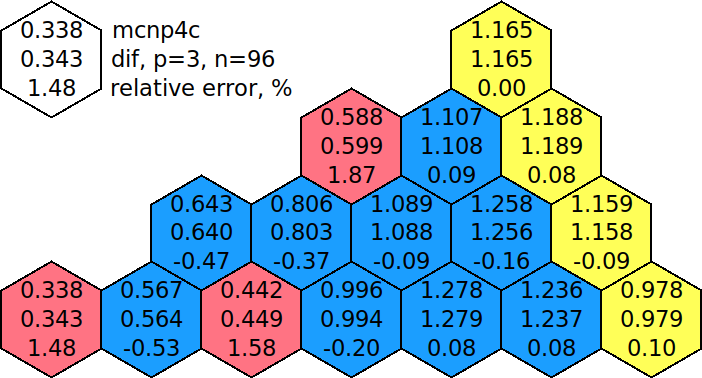
\includegraphics[width=0.7\linewidth]{dif.png}\\
	\caption{Power and error distributions using the diffusion model.}
	\label{fig:power_iaea_with_dif}
\end{center}
\end{figure}

\begin{figure}[htp]
\begin{center}
	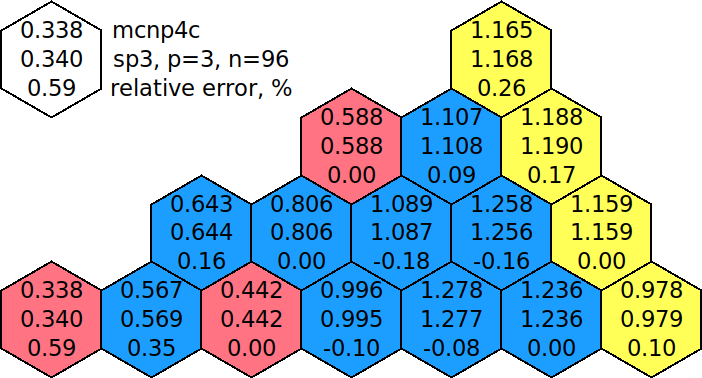
\includegraphics[width=0.7\linewidth]{sp3.png}\\
	\caption{Power and error distributions using the $\mathrm{SP_3}$ model.}
	\label{fig:power_iaea_with_sp3}
\end{center}
\end{figure}

\subsection{Solution of $\alpha$-spectral problem with delayed neutrons}

As a reference solution, we use the fine mesh solutions obtained using the transport $\mathrm{SP_3}$ model ($ p = 3, n = 96 $).
The $\alpha$-spectral problem results are shown in Table~\ref{tab:iaea_with_alpha_del}.

The calculation results for the first 10 eigenvalues are shown in Table~\ref{tab:iaea_with_alpha_del_10}.
The eigenvalues are well separated. 
The fundamental eigenvalue is negative and therefore the main harmonic will increase, while all others will attenuate. 
A regular mode of the reactor is thereby defined.
The value $\alpha = \lambda_1^{(\alpha)}$ determines the amplitude of neutron flux and is connected directly with reactor period in the regular mode.

\begin{table}[h]
\caption{The $\alpha$-eigenvalues.}
\label{tab:iaea_with_alpha_del}
\begin{center}
\begin{tabular}{c c r r r r r r}
\hline
$n$ & $p$ & $\alpha_{dif}$ & $\Delta_{dif}$ &$t$ &$\alpha_{sp_3}$& $\Delta_{sp_3}$&$t$ \\
\hline
	& 1	&$-$68.2268 &$-$66.8893& 0.01& $-$88.9461 &87.6086 &0.02\\
6	& 2	& $-$1.2810 & 0.0565& 0.05& $-$11.1554 & 9.8179 &0.19\\
	& 3	& $-$0.4506 & 0.8869& 0.18& $-$1.8063 & 0.4688 &0.65\\ 
\hline
	& 1	& $-$9.0267  &$-$7.6892& 0.05& $-$25.1658 &23.8283 &0.17\\
24& 2	& $-$0.4686  & 0.8689& 0.37& $-$1.9832 & 0.6457 &1.54\\
	& 3	& $-$0.4202  & 0.9173& 1.26& $-$1.3787 & 0.0412 &5.10\\ 
\hline
	& 1	& $-$0.7018  & 0.6357& 0.33& $-$4.9794 & 3.6419 &1.36\\
96& 2	& $-$0.4225  & 0.9769& 2.66& $-$1.3994 & 0.0619 &11.65\\
	& 3	& $-$0.4184  & 0.9191& 9.01& $-$1.3375 &    -- &38.16\\ 
\hline
Ref.&   & $-$1.3375  &       &     & $-$1.3375 \\ 
\hline
\end{tabular}
\end{center}
\end{table}

\begin{table}[h]
\caption{The eigenvalues $\alpha_i=\lambda_i^{(\alpha)}$ for $p=3, n=96$.}
\label{tab:iaea_with_alpha_del_10}
\begin{center}
\begin{tabular}{c r r}
\hline
$i$ & Diffusion & SP$_3$ \\
\hline
1& $-$0.418414021 &$-$1.337480417\\
2& 0.028108057    &   0.023799162\\
3& 0.028108075    &   0.023804256\\
4& 0.062814035    &   0.062218273\\
5& 0.062814041    &   0.062220971\\
6& 0.069514636    &   0.069228497\\
7& 0.073730817    &   0.073541211\\
8& 0.074126208    &   0.073987939\\
9& 0.075346220    &   0.075210662\\
10& 0.076266017   &   0.076175218\\
\hline
\end{tabular}
\end{center}
\end{table}

\section*{Acknowledgements}

This work was supported by the grant of the Russian Federation Government (\#~14.Y26.31.0013) and by the Russian Foundation for Basic Research (\#~18-31-00315).

\section*{References}
\begin{thebibliography}{9}
\bibitem{brantley2000simplified} Brantley P S, Larsen E W 2000 The simplified P3 approximation {\it Nuclear Science and Engineering} {\bf 134}, 1-21.

\bibitem{bell1970}
Bell G I, Glasstone S 1970 Nuclear Reactor Theory {\it Van Nostrand Reinhold Company}

\bibitem{stacey2007}
Stacey W M 2007 Nuclear Reactor Physics. {\it Wiley}

\bibitem{avvakumov2017spectral}
Avvakumov A V, Strizhov V F, Vabishchevich P N, Vasilev A O 2017 {\it Annals of Nuclear Energy} {\bf 99} 68-79

\bibitem{ryu2013fem}
Ryu E H, Joo H G 2013 {\it Annals of Nuclear Energy} {\bf 56} 194-207

\bibitem{chao1995}
Chao Y A, Shatilla Y A 1995 {\it Nuclear Science and Engineering} {\bf 121} 210-225

\bibitem{brenner2008}
Brenner S C, Scott L R 2008 The mathematical theory of finite element
methods {\it Springer}

\bibitem{logg2012}
Logg A, Mardal K A, Wells G 2012 The FEniCS book {\it Springer Science \& Business Media}

\bibitem{avvakumov2014}
Avvakumov A V, Vabishchevich P N, Vasilev A O 2014 {\it Vestnik
of the NEFU} {\bf 11} 7-18

\bibitem{avvakumov2015}
Avvakumov A V, Vasilev A O, Zakharov P E 2015 {\it Vestnik of
the NEFU} {\bf 4(48)} 35-44

\bibitem{bahabadi2016}
Bahabadi M H, Pazirandeh A, Mitra A 2016 {\it Annals of Nuclear Energy} {\bf 98} 74-80

\end{thebibliography}

\end{document}


